\chapter{Introduction}

\hrulefill

Although a large part of modern biology is devoted to uncovering the functions of the vast array of DNA, RNA and protein molecules that make up an organism, the concept of function remains surprisingly slippery. This can be best illustrated by the recent uproar surrounding the publication of the largest collection of datasets related to non-coding DNA to date by the ENCODE and modENCODE projects \citep{the_modencode_consortium_identification_2010, dunham_integrated_2012}. Famously, through integrating all of its datasets, the ENCODE consortium was able to grant 80.4\% of the nucleotides in the human genome a function; this figure, however, was quickly and hotly disputed \citep{dunham_integrated_2012,graur_immortality_2013}. It can be said that the function of a transcription factor (TF) is to bind DNA and regulate the expression of target genes; however, the complexity of combinatorial binding patterns and the sheer quantity of binding events, even in the model organism \emph{Drosophila}, which has a smaller and more compact genome than humans, suggest that TF function is complex and context-dependent \citep{biggin_animal_2011,kaplan_quantitative_2011,neph_expansive_2012,zinzen_combinatorial_2009}. One possible measure of biological function comes from the effect of natural selection, which, given a large enough population and free flow of alleles, should remove mutations that are detrimental to an organism and preserve those that allow for correct molecular function. Therefore, sequences or, by extension, TF binding events that are functional should be conserved by selection during evolution. In this thesis, I have applied the preceding hypothesis to the binding and function of two group B Sox proteins, a family of TFs that is both deeply conserved in animal evolution and shows complex interplays in binding patterns. Here I present an introduction to group B Sox proteins in vertebrates and insects, a review of previous studies that have used evolutionary comparisons to elucidate TF function and an overview of the experiments that I performed.  

\section{Glossary}
\begin{itemize}
	\item \textbf{Transcription factor (TF):} A protein whose primary function is to bind to DNA at specific recognition sites, either alone or in a complex with itself (as a homodimer) or other cofactors (as a heterodimer), in order to induce a positive or negative change in the level of transcription of a nearby gene.
	\item \textbf{Regulatory DNA:} Non-coding sequences of DNA that, when bound by the appropriate transcription factors, are necessary and sufficient to direct spatially and temporally specific expression patterns of nearby genes. Regulatory sequences may be located in intergenic DNA (upstream or downstream of genes) as well as in introns. Individual units of regulatory DNA are often referred to as enhancers or cis-regulatory elements (CRMs).
	\item \textbf{Transcription factor binding site (TFBS):} A small stretch of DNA, typically ranging from 6-12 nucleotides, that is recognized and bound by a transcription factor, often resulting in upregulation or downregulation of a nearby target gene. The preferred DNA sequence recognized by a particular TF is often referred to as a sequence motif; however, the sequences of individual TFBS instances can vary, a phenomenon known as degeneracy. Not all binding events of a TF to a TFBS result in a change in gene expression.
	\item \textbf{Target gene:} A gene whose regulatory DNA is bound by a particular TF. Genes whose expression has been demonstrated to change in response to TF binding are typically referred to as direct targets of that TF; however, TF binding at a target gene can also play an indirect role in gene regulation, for example through recruiting and stabilizing cofactors or changing the local chromatin environment.
\end{itemize}

\section{Group B Sox Proteins}
\emph{Sox} genes encode a deeply-conserved family of transcription factors (TFs) that serve as broad developmental regulators in metazoa. They are thought to have evolved in conjunction with the origin of multicellular animal life, as they are present in all animal genomes in which they have been searched for, including basal members such as sponges and placozoa \citep{jager_expansion_2006,jager_insights_2008,larroux_developmental_2006,phochanukul_no_2010,srivastava_trichoplax_2008}. Members of the Sox (Sry-related high-mobility-group box) family contain one highly conserved HMG (high-mobility group) DNA-binding domain, which typically shares greater than 50\% sequence homology to that of the mammalian testis-determining factor SRY \citep{bowles_phylogeny_2000,guth_having_2008,phochanukul_no_2010,sinclair_gene_1990}. They bind to DNA in the minor groove, recognizing variants of the motif A/TA/TCAAAG, and are known to induce DNA bending \citep{bowles_phylogeny_2000,ferrari_sry_1992,giese_hmg_1992}. Sox genes are classified into ten groups, A through J, based on HMG sequence and full-length protein structure \citep{schepers_twenty_2002}. Members of each subgroup are often expressed in overlapping patterns in particular subsets of tissues during development and play important roles in directing the correct differentiation of cells in those tissues; for example, in vertebrates, group B genes are expressed in the developing central nervous system and eye \citep{bergsland_sequentially_2011,kamachi_involvement_1998,uwanogho_embryonic_1995,wood_comparative_1999}, while group C genes are expressed in the kidney and pancreas \citep{huang_transcription_2013,sock_gene_2004,wilson_hmg_2005}, groups C, D and E are expressed in the skeleton and cartilage \citep{akiyama_transcription_2002,smits_transcription_????}, and group F genes are expressed in the developing vascular and lymphatic systems \citep{downes_sox18_????,matsui_redundant_2006}. Based on these observations and genomic studies that have identified many targets of various Sox proteins, it appears that the Sox family has evolved to regulate cell fate decisions in diverse tissue types across the animal phylogeny \citep{lefebvre_control_2007,whyte_master_2013}. While mammalian genomes contain multiple paralogues for most of these groups, invertebrates typically have far fewer Sox genes. Sequenced insect genomes, including that of Drosophila, typically contain one gene in each of groups C, D, E, and F, and four genes in group B, although occasional extra genes have originated in particular lineages (Figure 1.1) \citep{bowles_phylogeny_2000,phochanukul_no_2010}.\\

\begin{figure}
\centering
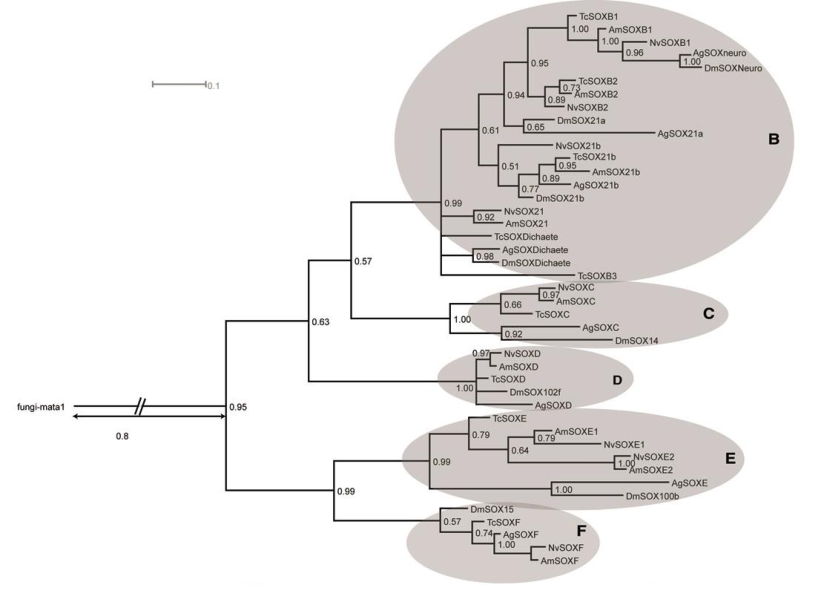
\includegraphics{fig1-1}
\caption{Rooted Bayesian phylogeny of representative insect Sox proteins. All species have four group B proteins except for \emph{T. castaneum}, which has an extra group B member (SoxB3), and all species have one member of each other subgroup except for the hymenopterans \emph{N. vitripennis} and \emph{A. mellifera}, which have undergone a gene duplication in group E. Figure reproduced from \citet{wilson_evolution_2008}. Abbreviations: Tc, \emph{Tribolium castaneum}; Am, \emph{Apis mellifera}; Nv, \emph{Nasonia vitripennis} Ag, \emph{Anopheles gambiae}; Dm, \emph{Drosophila melanogaster}.}
\label{Figure 1.1}
\end{figure}

Group B \emph{Sox} genes are some of the best characterized members of the \emph{Sox} family. In addition to being the most closely related \emph{Sox} genes to \emph{Sry}, they appear to have highly conserved functions throughout evolution \citep{collignon_comparison_1996,mckimmie_conserved_2005}. In mammals, group B \emph{Sox} genes have been implicated in stem cell pluripotency and self-renewal, ectoderm formation, neural induction, central nervous system (CNS) development, placode formation, and gametogenesis \citep{guth_having_2008}. A role for group B \emph{Sox} genes in neural development appears to be conserved throughout the higher metazoa, making \emph{Drosophila} an attractive system in which to study group B \emph{Sox} function and evolution more closely \citep{uwanogho_embryonic_1995,wood_comparative_1999,wegner_stem_2005}. Group B \emph{Sox} genes have also been analyzed at both sequence and expression levels in several species of invertebrates, showing strong evidence for functional conservation but also revealing a complex evolutionary history whose details are not fully resolved \citep{wilson_evolution_2008,mckimmie_conserved_2005,wei_identification_2010,pioro_expression_2006,zhong_parallel_2011}. There are four group B \emph{Sox} genes in the \emph{Drosophila melanogaster} genome: \emph{SoxNeuro (SoxN)}, \emph{Dichaete}, \emph{Sox21a}, and \emph{Sox21b} \citep{mckimmie_conserved_2005}. Of these, the most extensively studied to date are \emph{SoxN} and \emph{Dichaete}.\\

In vertebrates, group B \emph{Sox} genes are divided into two subgroups: group B1, which includes \emph{Sox1}, \emph{Sox2} and \emph{Sox3} \citep{collignon_comparison_1996}, and group B2, which includes \emph{Sox14} and \emph{Sox21} \citep{malas_isolation_1999,mckimmie_conserved_2005}. In the chicken, group B1 proteins act as transcriptional activators during development, while group B2 proteins act as transcriptional repressors \citep{uchikawa_two_1999,uchikawa_b1_2011}. Group B1 and B2 genes play opposing roles in the developing vertebrate CNS, with group B1 proteins conveying early neuroectodermal competence and maintaining neural precursors while group B2 proteins promote neuronal differentiation \citep{wegner_stem_2005,wegner_sox_2011}. Although it has been argued based on sequence orthology that \emph{SoxN} is a group B1 gene while \emph{Dichaete} is more closely related to the B2 subgroup \citep{bowles_phylogeny_2000,guth_having_2008,wegner_stem_2005,zhong_parallel_2011}, functional arguments place \emph{Dichaete} with the group B1 genes \citep{mckimmie_conserved_2005}. For example, \emph{Dichaete} specific mutant phenotypes in the \emph{Drosophila} CNS midline are rescued by expression of the mouse Sox2 protein, supporting the idea that both \emph{Dichaete} and \emph{SoxN} may be orthologous to vertebrate group B1 genes \citep{soriano_drosophila_1998}. Additionally, Dichaete is known to interact molecularly with the POU-domain protein Ventral veins lacking (Vvl), while mammalian Sox2 interacts with the POU protein Oct4 and can also interact with Vvl when expressed in the fly \citep{ambrosetti_synergistic_1997,archer_interaction_2011,bery_characterization_2013,ma_functional_2000,masui_pluripotency_2007,soriano_drosophila_1998,tanaka_interplay_2004}. Further functional data suggests that the B1-B2 division may not be functionally relevant in insects, as both \emph{Dichaete} and \emph{SoxN} play a number of complex roles during development that correspond to those played by vertebrate group B1 and B2 \emph{Sox} genes and that cannot be neatly divided into activator and repressor functions \citep{ferrero_soxneuro_2014}. Although it is difficult to assign orthology between vertebrate and insect group B \emph{Sox} genes due to their divergent evolutionary histories \citep{mckimmie_conserved_2005,wilson_evolution_2008,zhong_parallel_2011}, the similarities in the expression patterns and functions of \emph{Sox1}, \emph{Sox2} and \emph{Sox3} in vertebrates and \emph{SoxN} and \emph{Dichaete} in insects suggest that a combination of descent from a common group B \emph{Sox} ancestor and functional convergent evolution have shaped a deeply conserved yet complex relationship between these two sets of \emph{Sox} genes \citep{cremazy_<_2000,soriano_drosophila_1998,uwanogho_embryonic_1995,wood_comparative_1999,zhong_parallel_2011}. \\

Studies of \emph{in vivo} binding patterns of Sox proteins in mammals and flies have identified a large number of conserved orthologous targets, reinforcing the observation that the division of functions between group B paralogues cannot be simply translated from vertebrates to invertebrates. In the mouse, the group B1 genes \emph{Sox2} and \emph{Sox3} as well as the group C gene \emph{Sox11} are expressed in a successive fashion in the developing CNS; a recent ChIP-seq study examined binding patterns of Sox2, Sox3 and Sox11 in neural precursor cells (NPCs) and differentiated neurons. Although Sox2 and Sox3 are primarily responsible for maintaining NPCs, while Sox11 plays an opposite role by promoting the differentiation of neurons, all three proteins share a large proportion of their bound intervals and target genes. In addition to showing extensive common binding patterns, it appears that group B1 proteins expressed at earlier developmental timepoints can pre-bind target genes of later Sox proteins, priming them for later regulation by establishing bivalent chromatin marks without actually activating transcription \citep{bergsland_sequentially_2011}. In the case of \emph{Drosophila}, Dichaete and SoxN share large numbers of targets with both Sox2 and Sox11, demonstrating that they can play roles carried out by both group B and group C proteins in mammals and that their function cannot be easily split between the roles of maintaining neural precursors and promoting neural differentiation. Dichaete in particular shares a high number of orthologous targets with mouse Sox2, which is consistent with the functional rescue of \emph{Dichaete} mutant phenotypes achieved by expressing Sox2 protein \citep{soriano_drosophila_1998}. These shared targets are highly associated with transcriptional regulation and the generation of neurons, including genes involved in the neuroblast regulatory network, Notch signalling and neuroblast cell fate \citep{aleksic_role_2013}. Slightly fewer Sox2 targets are shared with core SoxN target genes; however, these genes are also strongly associated with CNS development. Interestingly, a much higher overlap in targets is observed between SoxN and Sox11, suggesting that SoxN in particular has a conserved role in neuronal differentiation and that some of its functions may have been co-opted by group C \emph{Sox} genes in mammals \citep{ferrero_soxneuro_2014}.\\

As with \emph{Sox1}, \emph{Sox2} and \emph{Sox3} in vertebrates, both \emph{Dichaete} and \emph{SoxN} are expressed in overlapping patterns in the \emph{Drosophila} CNS and are necessary for its normal development, although they do not show sequential expression as do \emph{Sox2} and \emph{Sox3} \citep{bergsland_sequentially_2011,buescher_formation_2002,cremazy_<_2000,girard_chromatin_2006,sanchez-soriano_regulatory_2000,shen_identifying_2013}. \emph{Dichaete} mutant embryos show axonal and midline defects, which can be rescued by expressing Dichaete (or mammalian Sox2) in the midline \citep{sanchez-soriano_regulatory_2000}. \emph{SoxN} mutant embryos also show axonal defects and loss of lateral neurons \citep{buescher_formation_2002,overton_evidence_2002}. In \emph{Drosophila}, neuroblasts delaminate from the neuroectoderm in three columns on either side of the midline: the medial, intermediate, and lateral columns. \emph{Dichaete} and \emph{SoxN} expression patterns partially overlap in these columns; \emph{Dichaete} is expressed from the midline outwards to the intermediate column, while \emph{SoxN} is excluded from the midline but is expressed from the medial column to the lateral column \citep{overton_evidence_2002} (Figure 1.2). \emph{SoxN/Dichaete} double mutants have more severe CNS defects than either single mutant; in particular, they show an increased loss of neuroblasts in the medial column in comparison to single mutants, which is where \emph{SoxN} and \emph{Dichaete} expression overlaps most strongly (Figure 1.3) \citep{buescher_formation_2002,overton_evidence_2002}.A similar effect is observed among mutants for the three vertebrate group B1 \emph{Sox} genes, where mice lacking \emph{Sox1} or \emph{Sox3} show only mild brain and spinal cord phenotypes, and neuroectoderm development is normal in \emph{Sox2} hypomorphs \citep{ferri_sox2_2004,guth_having_2008,nishiguchi_sox1_1998,rizzoti_sox3_2004,wegner_stem_2005}. In zebrafish, in which six group B1 genes are present, severe embryonic and CNS defects are only present in quadruple \emph{sox2/sox3/sox19a/sox19b} knockdowns \citep{okuda_b1_2010}. Such apparent redundancy is also observed with paralogous vertebrate \emph{Sox} genes in other subgroups, including the group C genes \emph{Sox4}, \emph{Sox11} and \emph{Sox12} and the group F genes \emph{Sox17} and \emph{Sox18} \citep{bhattaram_organogenesis_2010,matsui_redundant_2006}. These results strongly suggest functional compensation between Sox family members is widespread; however, the evolutionary driver for this phenomenon is not fully understood.\\

\begin{figure}
\centering
\includegraphics{fig1-2}
\caption{Dichaete and SoxN expression in the neuroectoderm of stage 10 \emph{D. melanogaster} embryos. Several planes of focus are shown. Dichaete is expressed in the ventral midline (green cells, indicated by white arrows) as well as the medial and intermediate columns of neuroblasts. SoxN is expressed with Dichaete in the medial and intermediate columns (yellow) and alone in the lateral column of neuroblasts (red). Figure reproduced from \citet{overton_phd}.}
\label{Figure 1.2}
\end{figure} 

\begin{figure}
\centering
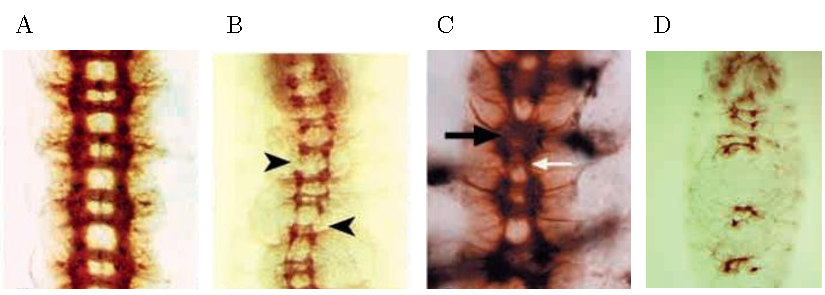
\includegraphics{fig1-3}
\caption{\emph{Dichaete/SoxN} double mutants show a more severe CNS phenotype than either single mutant. Flat preparation of stage 16 \emph{D. melanogaster} embryos stained for BP102 to show the axonal structure of the CNS. A.) Wild type embryo. B.) \emph{SoxN}-mutant (\emph{SoxNeuro\textsuperscript{U6-35}}) embryo. Arrowheads show lack of longitudinal staining in hemisegments. C.) \emph{Dichaete}-mutant (\emph{D\textsuperscript{r72}/Df}) embryo. The white arrow shows thinning of longitudinal connectives, and the black arrow shows fusion of commissural connectives. D.) \emph{SoxNeuro\textsuperscript{U6-35}/D\textsuperscript{r72}} double-mutant embryo. Longitudinal axons are almost completely absent and the neuropil shows frequent gaps. Figures reproduced from \citet{overton_evidence_2002} and \citet{soriano_drosophila_1998}.}
\label{Figure 1.3}
\end{figure}

In addition to functional compensation at the level of neural phenotypes, \emph{in vivo} binding and expression studies of Dichaete and SoxN in \emph{D. melanogaster} show that they have highly similar genome-wide binding patterns and share a large number of gene targets \citep{aleksic_role_2013,ferrero_soxneuro_2014}. Commonly bound gene targets cover many of the core functionalities of both Dichaete and SoxN, including over a hundred other TFs active in the CNS, the proneural genes of the \emph{achaete-scute} complex, \emph{Dr} and \emph{vnd}, which encode TFs involved in dorso-ventral patterning in the CNS \citep{zhao_genetic_2007}, and the neuroblast temporal identity genes \emph{svp}, \emph{hb}, \emph{Kr} and \emph{pdm2} \citep{ferrero_soxneuro_2014,isshiki_drosophila_2001,maurange_brainy_2005}. Previous \emph{in vivo} binding studies of Dichaete have provided evidence that it can bind to highly occupied target (HOT) regions, which are areas of the genome that are bound commonly by many TFs and are associated with open chromatin \citep{aleksic_role_2013,kvon_hot_2012}. A role for Dichaete as a modulator of DNA architecture that supports the binding of other TFs has also been proposed \citep{russell_dichaete_1996}. Together, these suggest that the binding patterns of group B Sox proteins, like many other developmental TFs that have been studied in the fly, may be strongly influenced by patterns of chromatin accessibility in addition to recognition of specific sequence motifs \citep{ferrero_soxneuro_2014,macarthur_developmental_2009}. However, it is unknown to what extent the chromatin environment drives Dichaete and SoxN binding or if all binding events in open chromatin are associated with gene regulation.\\

Further complicating the picture, not only do Dichaete and SoxN share many targets, they also display a complex pattern of compensatory binding in each other’s absence. DamID experiments examining SoxN binding in \emph{Dichaete} mutants and vice versa have identified loci where one TF can compensate for the other’s absence by increasing its own binding. In addition, there are loci where the loss of one of these two Sox proteins appears to result in a loss of binding by the other (Figure 1.4). These observations suggest that Dichaete and SoxN can compensate for one another in some instances, but that they are also dependent on one another in order to function correctly in others. Furthermore, in some genomic locations the loss of one TF does not affect the binding of the other, indicating that their functions at certain loci are independent \citep{ferrero_soxneuro_2014}. Considering the deep conservation of \emph{Dichaete} and \emph{SoxN} as paralogues throughout the insects \citep{mckimmie_conserved_2005,wilson_evolution_2008}, it remains unclear why evolution has maintained these two partially redundant proteins. \\

\begin{figure}
\centering
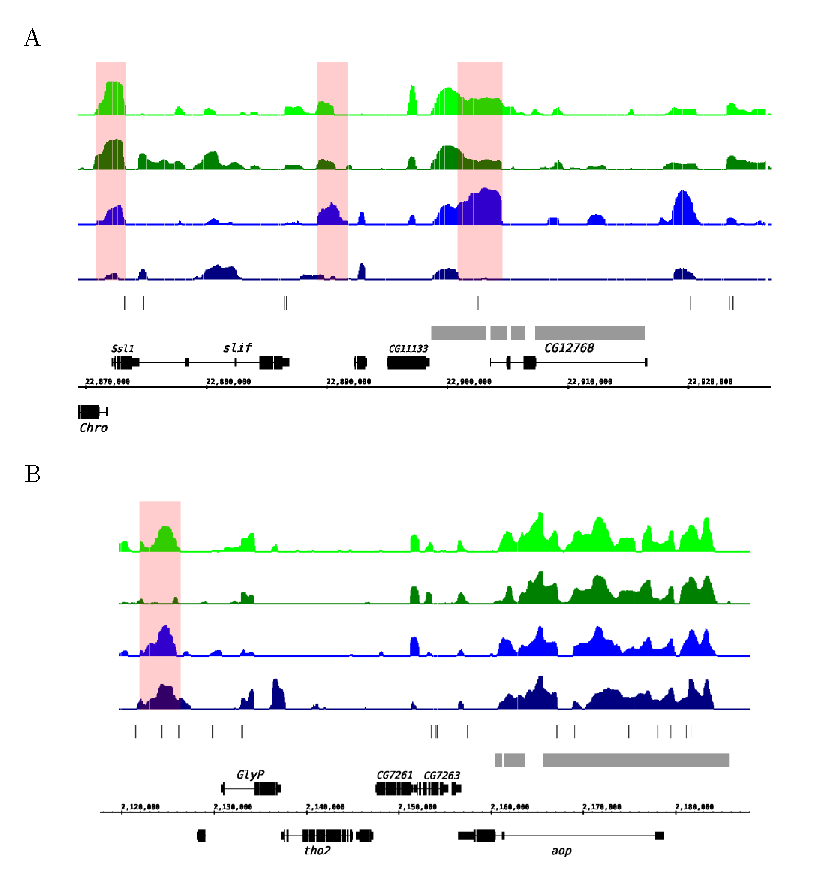
\includegraphics{fig1-4}
\caption{Reciprocal binding compensation by Dichaete and SoxN. Tracks show, from the bottom, gene models (black), known enhancers (gray), Sox motifs (gray), SoxN DamID in wild type (dark blue), SoxN DamID in \emph{Dichaete} mutant background (blue), Dichaete DamID in wild type (dark green), Dichaete DamID in \emph{SoxN} mutant background (light green). A.) Pink boxes show SoxN compensating for Dichaete binding. Dichaete is normally bound at these loci while SoxN is not; however, in a \emph{Dichaete} mutant background, SoxN binds here (blue). B.) The pink box shows Dichaete compensating for SoxN binding. SoxN is normally bound at this locus while Dichaete is not; however, in a \emph{SoxN} mutant background, Dichaete binds here (light green). Figures reproduced from \citet{ferrero_soxneuro_2014}.}
\label{Figure 1.4}
\end{figure}

The generation of new paralogues through gene duplications events has occurred frequently during metazoan evolution and is a major driver of increased complexity in genetic regulatory networks \citep{larroux_genesis_2008}. The theoretical expectation after gene duplication has occurred is that the new paralogue experiences reduced selective pressure, as it is essentially a redundant copy of the original gene. This opens the door for the accumulation of mutations, which can lead to loss of function and transformation of one of the new paralogues into a pseudogene. Alternatively, if favorable mutations occur, then subfunctionalization, in which the role of the original gene is divided amongst the new paralogues either by functional domain or by spatial/temporal expression pattern, or neofunctionalization, in which the new copy acquires functions that did not belong to the original gene, can occur \citep{force_preservation_1999,lynch_evolutionary_2000}. One well-studied example of subfunctionalization and neofunctionalization is the evolution of \emph{Hox} genes, which code for a highly-conserved family of transcription factors that are primarily involved in establishing segmental identity along the anterior-posterior (AP) axis \citep{kappen_evolution_1993}.\\ 

Paralogous \emph{Hox} genes have specific, though sometimes overlapping, expression domains along the AP axis and provide spatial information to downstream genes in order to direct the development of appropriate segmental morphology. In vertebrates, \emph{Hox} genes have undergone tandem duplications followed by multiple whole-group duplications to result in in four \emph{trans}-paralogous clusters, located on four different chromosomes \citep{foronda_function_2009,maconochie_paralogous_1996}. Interestingly, \emph{trans}-paralogous genes in the same relative positions (e.g. \emph{Hoxa1} and \emph{Hoxb1}) have retained greater similarities in sequence and expression patterns than \emph{cis}-paralogous genes in each cluster (e.g. \emph{Hoxa1} and \emph{Hoxa2}). Although \emph{Hox} single mutants typically do show specific phenotypes, there is some evidence for partial redundancy between \emph{trans}-paralogues such as \emph{Hoxa3} and \emph{Hoxd3} \citep{greer_maintenance_2000}. In contrast, in both flies and vertebrates, \emph{Hox} paralogues that arose through linear gene duplications have acquired largely unique expression domains and functions. Mutant phenotypes associated with each paralogous member of a single \emph{Hox} cluster appear in specific domains along the AP axis that correspond to the expression patterns of that member \citep{maconochie_paralogous_1996}. ChIP-chip experiments in \emph{Drosophila} have confirmed that Hox proteins show a high level of \emph{in vivo} specificity in their binding targets, although this specificity is likely to arise from a combination of specific DNA recognition sequences and the presence of unique combinations of cofactors \citep{hueber_comparative_2007,hueber_shaping_2008,mann_chapter_2009}.\\

Such specialization of paralogous genes after duplication has been suggested to drive the evolution of new gene regulatory modules, which can, in turn, facilitate adaptability and evolutionary innovation \citep{espinosa-soto_specialization_2010}. However, cases of genetic redundancy appear be conserved as a stable evolutionary state more often than theoretically predicted and in many different taxa \citep{lynch_probability_2001,vavouri_widespread_????}. Redundancy between a pair of forkhead transcription factors, \emph{pes-1} and \emph{fkh-2}, has been shown to be conserved between two species of nematode, \emph{C. elegans} and \emph{C. briggsae} \citep{molin_evolutionary_2000}. In yeast, persistent functional redundancy among pairs of duplicated genes, measured in terms of overall fitness, appears to be widespread \citep{dean_pervasive_2008}. In contrast to the phenotypic and regulatory target specificity seen for \emph{cis}-paralogous \emph{Hox} genes in insect and vertebrates, functional redundancy in \emph{Sox} genes from the same subgroup seems to be a common theme across evolution, with paralogues in multiple subgroups and in many different taxa showing overlapping patterns of expression and a lack of strong single-mutant phenotypes \citep{bhattaram_organogenesis_2010,buescher_formation_2002,ferri_sox2_2004,guth_having_2008,matsui_redundant_2006,nishiguchi_sox1_1998,okuda_b1_2010,overton_evidence_2002,rizzoti_sox3_2004,uchikawa_b1_2011,uwanogho_embryonic_1995,wegner_stem_2005,wood_comparative_1999}.\\ 

One possible explanation for the compensation shown by \emph{Dichaete} and \emph{SoxN} is to provide greater regulatory robustness to the developing CNS; it has been argued that functional redundancy may be a general mechanism for promoting robustness in genetic regulatory networks  \citep{nowak_evolution_1997,tautz_redundancies_1992,wagner_distributed_2005,wagner_gene_2008}. If regulation of the developing neuroectoderm represents the ancestral group B \emph{Sox} function, then the unique, and sometimes opposing, roles of \emph{Dichaete} and \emph{SoxN} may be examples of partial neofunctionalization in the insects \citep{ferrero_soxneuro_2014}. Both genes have independent functions; for example, \emph{Dichaete} is expressed in unique domains, including the embryonic brain and hindgut, where it has important regulatory functions \citep{sanchez-soriano_regulatory_2000}. Similarly, \emph{SoxN} is prominently expressed in the ectoderm of the late embryo, where it has roles in cuticle patterning that are only partially compensated for by \emph{Dichaete} \citep{overton_drosophila_2007}. If both the unique and common functions of the two proteins are conserved by natural selection, one would expect to find evidence of similar functionality and binding patterns throughout the insect phylogeny. In order address this question, I set out to examine the genome-wide \emph{in vivo} binding patterns of both Dichaete and SoxN in four species of \emph{Drosophila}. My goal was both to understand the evolutionary dynamics of group B Sox binding, including the rates of gain and loss of binding sites, as well as to test whether Dichaete and SoxN binding at common gene targets and specific binding at unique targets are equally conserved. In order to do so, I used a strategy of comparative binding analysis, drawn from several previous evolutionary studies of transcription factor binding in both \emph{Drosophila} and vertebrates.


\section{Comparative studies of transcription factor binding}
The importance of regulatory DNA in development, disease and evolution is widely accepted and becoming a key focus for genomics as large-scale studies such as the ENCODE project attempt to map diverse elements of the non-coding genome \citep{dunham_integrated_2012,gordon_tempo_2012,neph_expansive_2012,wray_evolutionary_2007}. One of the major roles of regulatory DNA is to bind transcription factors and, together with other genomic elements such as promoters, to direct gene expression in a temporally and spatially specific manner. In the model organism \emph{Drosophila melanogaster}, significant strides have been made towards understanding how multiple inputs are integrated to determine transcription factor occupancy in the nucleus, and how, in turn, combinatorial rules of transcription factor binding describe functional regulatory elements \citep{kaplan_quantitative_2011,li_role_2011,zinzen_combinatorial_2009}. However, the primary methods for determining transcription factor binding, both \emph{in vivo} and \emph{in silico}, suffer from difficulties in distinguishing between true functional events and biological noise, resulting in high numbers of potential false positives and making it difficult to tease apart underlying regulatory networks \citep{biggin_animal_2011,fisher_dna_2012,macarthur_developmental_2009}. One potential way to circumvent this problem is via comparative studies of transcription factor binding in multiple \emph{Drosophila} species, which facilitate the use of patterns of conservation to identify functional features of the regulatory genome as well as an analysis of the evolutionary dynamics of transcriptional regulation.\\

A number of different techniques for directly or indirectly studying genome-wide transcription factor binding patterns in \emph{Drosophila} are available. Two of the primary \emph{in vivo} techniques are ChIP (chromatin immunoprecipitation) and DamID, the latter based on DNA methylation by a tethered DNA adenine methyltransferase (dam) \citep{greil_[16]_2006} (Figure 1.5). Both of these techniques can be combined with either hybridization to a microarray or high-throughput sequencing in order to identify preferentially-bound regions genome-wide \citep{aleksic_chiping_2009,van_steensel_chromatin_2001}; however, because arrays are generally not commercially available for non-model species and the cost of sequencing has dropped significantly in the last decade, sequencing has become the method of choice for most comparative studies. With the publication of the modENCODE data in 2010 \citep{the_modencode_consortium_identification_2010}, a large number of ChIP-chip and ChIP-seq datasets from \emph{Drosophila melanogaster} were made publicly available; at the time of writing, the modMine database, which houses the modENCODE datasets, contains 279 entries for ChIP-chip and ChIP-seq datasets for transcription factor binding as well as chromosomal proteins and histone modifications in \emph{D. melanogaster} \citep{contrino_modmine:_2011}. In addition, a more focused study on the binding of 31 transcription factors involved in early embryonic patterning, along with matching chromatin accessibility data, are available from the Berkeley Drosophila Transcriptional Network Project \citep{macarthur_developmental_2009}. The availability of these datasets, as well as data-processing tools, quality control guidelines and experimental best practices from the modENCODE consortium \citep{landt_chip-seq_2012,trinh_cloud-based_2013}, provides a valuable resource for researchers wishing to undertake comparative studies in other \emph{Drosophila} species. ChIP-seq experiments have been successfully performed with transcription factors in \emph{D. simulans, D. yakuba, D. erecta, D. ananassae, D. pseudoobscura} and \emph{D. virilis} \citep{bradley_binding_2010,he_high_2011,paris_extensive_2013,villar_evolution_2014}, representing an evolutionary span of approximately 40 million years.\\

\begin{figure}
\centering
\includegraphics{fig1-5}
\caption{Overview of ChIP-seq and DamID-seq pipelines. A.) In ChIP-seq, embryos are first crosslinked with formaldehyde, and then chromatin is isolated and fragmented. An antibody specific to the TF of interest is used to enrich the sample for bound DNA fragments; mock IP and input chromatin controls are prepared in parallel. After reversal of crosslinks, the DNA is purified and sequenced, and reads are mapped to the reference genome. TFs are represented by orange hexagons, specific antibodies in red and control antibodies for mock IPs in blue. B.) In DamID-seq, two transgenic lines are created: one expressing a TF-Dam fusion and one expressing a Dam-only control. DNA is isolated from embryos of each line and digested with \emph{Dpn}I, which cuts GATC sequences when the A is methylated. The resulting DNA is purified and sequenced, and rads are mapped to the reference genome. The top trace represents that Dam-TF profile and the bottom trace the Dam-only control profile. TFs are represented by orange hexagons, the Dam enzyme by a blue diamond, GATC motifs by red lines, and methylated adenine residues by gray ovals. Figure reproduced from Carl and Russell (in press).}
\label{Figure 1.5}
\end{figure}

One of the most fundamental questions that comparative transcription factor binding studies can ask is whether, and to what extent, individual binding events are conserved between different species. Several studies, focusing on different transcription factors and using different sets of species, have independently attempted to estimate binding conservation as well as the rate of binding site turnover in \emph{Drosophila}. One of the first of these used ChIP-chip to measure genome-wide binding of the transcription factor Zeste. ChIP-chip was performed only in \emph{D. melanogaster}, and the resulting binding intervals were aligned against the genomes of \emph{D. simulans, D. erecta} and \emph{D. yakuba} \citep{moses_large-scale_2006}. Since \emph{in vivo} binding data was only available for one species, an analysis of quantitative differences in binding between species was not possible; instead, the authors considered binding as a binary state based on called peaks. Using a conservative approach, only binding intervals identified in \emph{D. melanogaster} that could be unambiguously aligned to orthologous sequences in each of the other species were included, and the analysis was further restricted to those intervals containing matches to a Zeste binding motif positional weight matrix (PWM). Nonetheless, the authors found that at least 5\% of Zeste binding sites identified in \emph{D. melanogaster} were not conserved in the other species they examined, implying that those sites were either gained in the \emph{D. melanogaster} lineage or lost in the other lineages since the divergence of the \emph{melanogaster} sub-group \citep{moses_large-scale_2006}.\\

Several more recent studies employing ChIP-seq to measure transcription factor binding in multiple species of \emph{Drosophila} generated broadly similar estimates of binding site conservation. Bradley and colleagues examined binding of 6 transcription factors involved in anterior-posterior (AP) patterning in the early embryo (Bicoid (Bcd), Hunchback (Hb), Kruppel (Kr), Giant (Gt), Knirps (Kni) and Caudal (Cad)) in the closely-related species \emph{D. melanogaster} and \emph{D. yakuba} \citep{bradley_binding_2010}. A subsequent experiment by the same group expanded the phylogenetic distance by measuring the binding of four of these factors (Bcd, Gt, Hb and Kr) in the same two species along with \emph{D. pseudoobscura} and \emph{D. virilis} \citep{paris_extensive_2013}. A third study focused on the mesodermal regulator Twist in six species: \emph{D. melanogaster, D. simulans, D. yakuba, D. erecta, D. ananassae} and \emph{D. pseudoobscura}, which span approximately 25 million years of evolutionary time \citep{he_high_2011}. Each of these studies considered both presence/absence of peaks in each species as well as quantitative changes in binding strength (Figure 1.6).\\ 

\begin{figure}
\centering
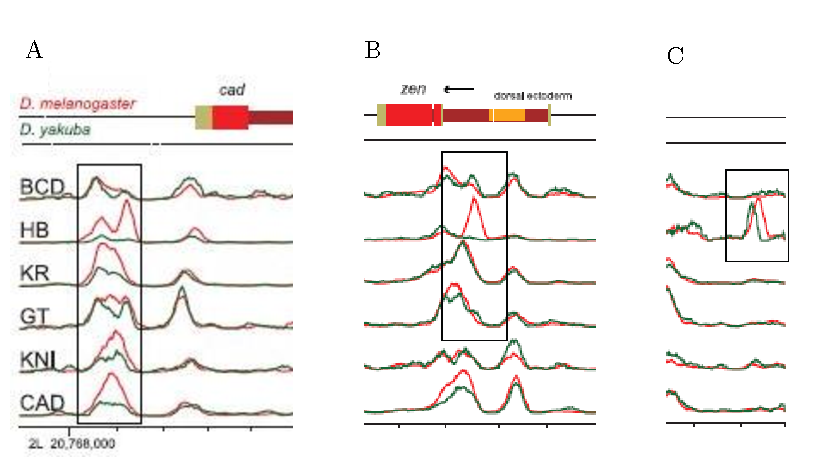
\includegraphics{fig1-6}
\caption{Examples of quantitative and qualitative changes in binding between five AP factors in \emph{D. melanogaster} (red) and \emph{D. yakuba} (green). A.) Examples of quantitative changes in binding strength between species with peak location conserved for several factors. B.) An example of the complete gain and loss of a peak between species for the factor Hb. C.) An example of a shift in binding site location between species with peak strength conserved for the factor Hb. Figure reproduced with modifications from \citet{bradley_binding_2010}.}
\label{Figure 1.6}
\end{figure}

Bradley \emph{et al.} found that, for each of the 6 factors studied, between 1\% and 15\% of peaks that were identified in one species were absent in the other. They measured quantitative binding divergence by calculating the genome-wide correlations between binding strength at all peaks for each factor in \emph{D. melanogaster} and \emph{D. yakuba}; these values ranged from 0.57 – 0.75 for peaks at genes not known to be regulated by the AP patterning factors and were higher at known target genes \citep{bradley_binding_2010}. In similar pairwise comparisons between binding strengths of peaks in \emph{D. melanogaster} and \emph{D. pseudoobscura}, the correlations ranged from 0.37 for Gt to 0.64 for Kr, reflecting the greater phylogenetic distance between the two species \citep{paris_extensive_2013}. In the case of Twist, around 80\% of peaks identified in \emph{D. melanogaster} were found to be conserved in \emph{D. simulans} and \emph{D. yakuba}, with the percentage decreasing to around 60\% for \emph{D. pseudoobscura}. The authors measured quantitative divergence by computing the number of peaks whose binding strength changed between \emph{D. melanogaster} and each other species; this ranged from around 10\% to 35\% of total peaks \citep{he_high_2011}. One common finding among these studies, as well as two others that focused on the insulator proteins CTCF and BEAF-32 \citep{ni_adaptive_2012,yang_beaf-32_2012}, is that differences in binding between species, measured either qualitatively or quantitatively, increase with the phylogenetic distance of the species being compared, prompting the hypothesis that binding divergence may follow a molecular clock mechanism \citep{he_high_2011}.\\

Besides simply estimating rates of binding conservation and divergence, comparative studies of transcription factor binding can identify new features of transcription factor function by considering differences in binding conservation relative to genomic annotations or patterns of binding by other factors. This type of analysis builds on the hypothesis that functional sites will be subject to purifying selection and thus will be preferentially conserved. One way to test this hypothesis is to evaluate conservation at a set of well-characterized functional regulatory elements. For example, peaks for AP patterning regulators are more conserved at known AP target genes compared to all genes, and peaks for Twist binding are highly conserved at regulatory elements that are known Twist targets \citep{bradley_binding_2010,he_high_2011,paris_extensive_2013}. Additionally, the most highly conserved Twist peaks show an enrichment near genes that are down-regulated in \emph{twist} mutants as well as genes that are annotated with Gene Ontology (GO) functions related to Twist's developmental role, both of which are also indicators of function. Clustered Twist sites assigned to the same gene are significantly more likely to be conserved than singleton sites assigned uniquely to a gene. This effect was observed up to an inter-peak distance of 5 kb, leading the authors to suggest that Twist binding to shadow enhancers might also have an effect on ensuring robustness of gene expression patterns \citep{he_high_2011}. In the case of AP transcription factors, Paris \emph{et al.} found that peaks in regions that were commonly bound by more than one factor were better conserved than those where only one factor bound, suggestive of a role for combinatorial binding between AP factors \citep{paris_extensive_2013}.\\

It is also possible to examine the effect of sequence level conservation on transcription factor binding. Both the two AP factor studies and the Twist study described above show that, while overall sequence conservation in bound regions does not correlate strongly with binding divergence, conservation of short sequence motifs within binding intervals does show some correlation with binding divergence \citep{bradley_binding_2010,he_high_2011,paris_extensive_2013}. He \emph{et al}. found that Twist peaks present in all four species studied had significantly more fully-conserved Twist motifs than peaks that were only present in \emph{D. melanogaster}. Similarly, the quality of Twist motifs present in peaks was also correlated with quantitative changes in binding strength between species. However, changes in motif quality alone do not explain all of the observed binding divergence in any of the cases studied, suggesting that other factors are at play in shaping binding patterns. After observing that not all losses of Twist binding could be attributed to a corresponding loss of a Twist motif, the authors decided to investigate whether other factors acting as binding partners for Twist had an effect on the conservation of its binding. A search for motifs that were significantly more conserved in highly-conserved Twist peaks compared to divergent Twist peaks or the background genome yielded two transcription factors known to act together with Twist: Snail and Dorsal. For Twist peaks in one species containing a Snail or Dorsal motif in addition to a conserved Twist motif, loss of the partner motif was sufficient to explain loss of Twist binding in another species in 19\% of cases. Furthermore, the top ten motifs identified in Twist binding intervals explained 49\% of losses of Twist binding despite conservation of a Twist motif. These findings go one step beyond a simple search for enriched motifs, identifying those that have a functional effect on binding patterns. Integration of an evolutionary analysis of gains and losses of Twist binding with a search for conserved co-occurring motifs led to both the validation of known Twist co-regulators such as Dorsal and Snail as well as the identification of new factors that could potentially bind to enhancers with Twist in a combinatorial manner to direct specific patterns of gene expression during development \citep{he_high_2011}.\\

By studying 6 different transcription factors, Bradley \emph{et al.} were in a unique position to examine the relationships between quantitative binding divergence for different factors across the genome. By performing principal component analysis (PCA) on regions bound by any factor, they found both a strong correlation between quantitative changes in binding strength across all factors (explaining 38\% of all binding divergence between \emph{D. melanogaster} and \emph{D. yakuba}) as well as both positive and negative correlations between changes in the binding of specific pairs of factors. For example, increases in binding of Giant, a repressor, were correlated with decreases in binding of Hunchback, an activator. A search for sequence motifs that were associated with the correlated binding divergence of all the AP factors revealed a CAGGTAG binding motif for the zygotic transcriptional activator Zelda \citep{bradley_binding_2010}. This strong association between AP factors and Zelda was later confirmed and extended into the more distant species \emph{D. pseudoobscura} and \emph{D. virilis} \citep{paris_extensive_2013}. Zelda has since been shown to be a key factor in establishing regulatory regions in the early embryo that will be active later in development, and it has been suggested that it plays an important role in shaping the chromatin landscape during zygotic genome activation \citep{harrison_zelda_2011,satija_tagteam_2012}. This example highlights a case where patterns of binding conservation for one set of transcription factors illuminated a new functional role for a different protein as well as a general feature of \emph{Drosophila} embryonic development.\\

In contrast to \emph{Drosophila}, comparative studies of transcription factor binding in vertebrate species show that binding patterns appear to have diverged much more over equivalent phylogenetic distances. The majority of binding sites of tissue-specific TFs in human, mouse, dog, opossum and chicken are species-specific, despite the highly-conserved DNA binding preferences of the orthologous proteins \citep{odom_tissue-specific_2007,schmidt_five-vertebrate_2010}. Even among closely-related mouse and rat species, TF binding patterns show less similarities than among \emph{Drosophila} species separated by similar periods of evolutionary time \citep{stefflova_cooperativity_2013}. Potential explanations for these discrepancies include the vast differences in genome size and density of functional elements between vertebrates and \emph{Drosophila} and the larger effective population size of insects in comparison to vertebrates, which tends to make natural selection more effective \citep{villar_evolution_2014}. Remarkably, mice carrying a copy of human chromosome 21 show TF binding patterns on that chromosome that recapitulate those seen in humans, rather than on the orthologous mouse chromosome 16, demonstrating that species-specific differences largely stem from the \emph{cis}-regulatory code itself, rather than other factors in the nuclear environment \citep{wilson_species-specific_2008}.\\

The degree of conservation of binding events in \emph{Drosophila} makes it a particularly suitable model system in which to study the evolution of regulatory DNA and to deduce information about TF function from evolutionary comparisons. In addition, the amenability of \emph{Drosophila} to molecular techniques and genetic manipulation, as well as the publication of the sequenced genomes and phylogenetic relationships of twelve \emph{Drosophila} species \citep{clark_evolution_2007} and the ongoing community efforts to sequence more species make the fruit fly a compelling model in which to conduct comparative studies of transcription factor binding. With this in mind, I chose to study the binding patterns of the two group B Sox proteins Dichaete and SoxN in four species of \emph{Drosophila}: \emph{D. melanogaster, D. simulans, D. yakuba} and \emph{D. pseudoobscura}. These four species span divergence times from approximately two million years to 25 million years, allowing for a range of evolutionary comparisons, yet their genomes are close enough for accurate alignment, which is critical for a comparative binding analysis \citep{russo_molecular_1995} (Figure 1.7). I aimed to use such an analysis to shed new light on the functional and evolutionary dynamics of group B Sox binding in \emph{Drosophila}.

\begin{figure}
\centering
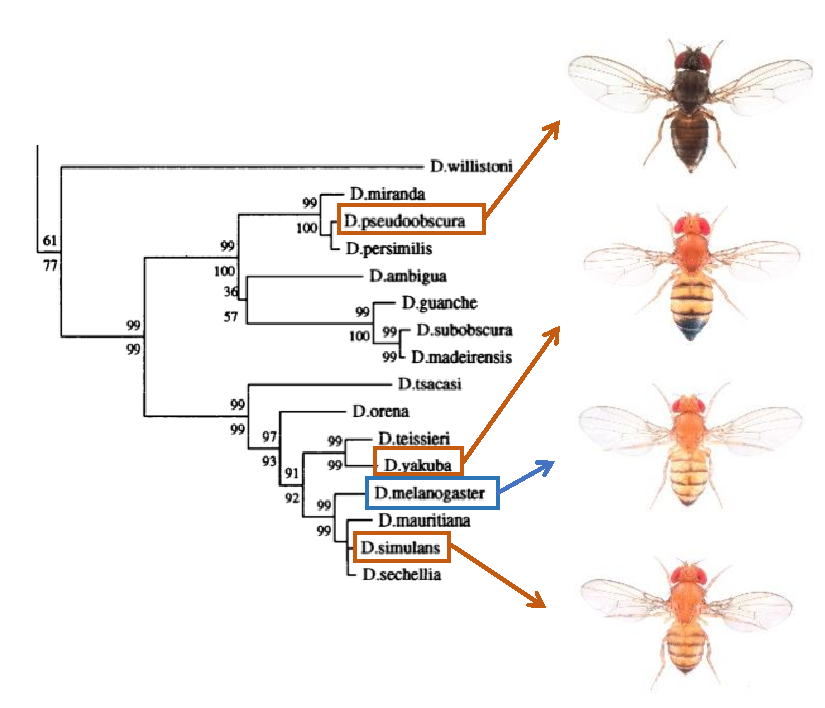
\includegraphics{fig1-7}
\caption{Phylogenetic relationship of \emph{Drosophila} species used in this thesis. The reference species, \emph{D. melanogaster}, is highlighted in the blue box. All non-model species are highlighted in red boxes. \emph{D. melanogaster, D. simulans} and \emph{D. yakuba} are located in the \emph{melanogaster} subgroup, while \emph{D. pseudoobscura} falls into the \emph{obscura} subgroup. The phylogenetic tree is a neighbor-joining tree based on \emph{Adh} nucleotide sequences from each species and is reproduced from \citet{russo_molecular_1995}. The confidence probability is shown above each branch, and the bootstrap confidence level from 1000 replications is shown below each branch. \emph{Drosophila} images are by Nicolas Gompel (\url{http://www.ibdml.univ-mrs.fr/equipes/BP_NG/Illustrations/melanogaster\%20subgroup.html}).}
\label{Figure 1.7}
\end{figure}

\section{Overview of experiments}
The main questions that I set out to answer during my Ph.D. can be summarized as follows:
\begin{enumerate}
	\item Where do Dichaete and SoxN bind in the genomes of \emph{D. simulans, D. yakuba} and \emph{D. pseudoobscura}, and what proportion of those binding sites are conserved with \emph{D. melanogaster}?
	\item Are there certain categories of binding sites that are more highly conserved across the drosophilids than others, and what can this tell us about Dichaete and SoxN function in invertebrates? Specifically, are sites that are commonly bound by both TFs equally conserved as those that are only bound by one?
	\item To what extent do patterns of chromatin accessibility differ between \emph{D. melanogaster} and \emph{D. pseudoobscura}, and what is the relationship between open chromatin and group B Sox binding?
\end{enumerate}

In order to address the first question, I initially set out to perform ChIP-seq for Dichaete and SoxN in all four species of interest. After verifying the similarities between Dichaete and SoxN expression patterns in each species via immunohistochemistry, I performed ChIP-PCR in each species and ChIP-chip in \emph{D. melanogaster} to test the performance of the antibodies against the two TFs in immunoprecipitations. Although the initial results were promising, two attempts at ChIP-seq for Dichaete failed to produce biological replicates with any significant, reproducible enrichment. The data from these preliminary experiments are presented in Chapter 3. After deciding that the ChIP-seq data was too noisy for any useful further analysis, I changed my experimental strategy and focused on performing DamID-seq for both Dichaete and SoxN in all four species. My first task was to create transgenic lines carrying Dichaete-Dam, SoxN-Dam and Dam-only constructs in each species; the details of this work are described in the methods section (Chapter 2). I then successfully carried out DamID-seq for Dichaete in \emph{D. melanogaster, D. simulans, D. yakuba} and \emph{D. pseudoobscura}, and for SoxN in \emph{D. melanogaster} and \emph{D. simulans}. In \emph{D. pseudoobscura}, I was unable to generate a SoxN-Dam line, while in \emph{D. yakuba} the DamID experiment failed, possibly due to a mutation in the transgenic SoxN sequence. A presentation of the DamID-seq datasets and a functional analysis of the binding patterns of the two TFs in each species can be found in Chapter 4.\\

Next, I compared the binding patterns of Dichaete-Dam and SoxN-Dam on both qualitative and quantitative levels in pairwise comparisons, and, in the case of Dichaete, in a three-way comparison between species. This allowed me to identify binding intervals that are unique to one species or conserved between two, three or four species. The detailed analysis of group B Sox binding conservation is presented in Chapter 5. In this section, I also address the second major question of my thesis. I examined differences in the rate of binding conservation between binding intervals associated with certain functional categories, such as those overlapping known enhancers or previously-identified Dichaete and SoxN target genes and core intervals. I also integrated the \emph{in vivo} binding data with the genome sequences available in all four species to search for Sox motifs within bound intervals and analyzed the relationship between the number, quality and sequence conservation of Sox motifs and binding conservation. Finally, I considered the rates of conservation of common binding by Dichaete and SoxN versus unique binding by either TF. In order to do so, I first performed a quantitative differential analysis of Dichaete and SoxN binding in both \emph{D. melanogaster} and \emph{D. simulans}, resulting in the detection of intervals that are commonly bound or uniquely bound in either one or both species. This allowed me to identify a strong relationship between common binding by both TFs and binding conservation, supporting the prior evidence for common regulation of many targets, as well as to examine the functions of potential targets that are uniquely bound by each TF across multiple species.\\

In order to address the third question, the role of chromatin accessibility in directing group B Sox binding and its differences between species, I performed FAIRE-seq in \emph{D. pseudoobscura} embryos collected at five developmental stages. A detailed description of the \emph{D. pseudoobscura} staging process as well as the FAIRE-seq protocol can be found in Chapter 2. These datasets, as well as a functional analysis of the accessible regions that I identified, are presented in Chapter 6. I used publicly-available ChIP-seq datasets for several TFs in \emph{D. pseudoobscura} to investigate the relationship between accessible chromatin identified by FAIRE and TF binding, as well as examining the correlation between FAIRE accessibility and Dichaete binding as identified by DamID in \emph{D. pseudoobscura}. A comparison of my FAIRE datasets with several chromatin accessibility datasets in \emph{D. melanogaster} embryos revealed that the \emph{D. pseudoobscura} FAIRE data may suffer from a lack of sensitivity, which could be due to technical problems during the chromatin preparation stage. Nonetheless, I was able to use these data to find significant associations between conserved Dichaete binding and open chromatin, supporting a role for chromatin accessibility not only in determining TF binding patterns but also in maintaining them during evolution.\\

As reviewed here, the importance of regulatory DNA during evolution has been increasingly recognized and studied over the last decade. However, conservation or divergence of regulatory regions can occur on several levels, and it is important to consider all of them in order to build a comprehensive picture of the function and evolution of transcriptional regulation. The central dogma of molecular biology often describes DNA as a language that must be read in order to produce RNA and proteins \citep{gerstein_what_2007}, and this linguistic metaphor has been extended to create more complex models of molecular grammar \citep{searls_linguistic_1997,searls_reading_2001,searls_language_2002}. Although regulatory DNA is not typically transcribed or translated itself, it can also be considered to have a type of grammar. If we consider an enhancer as a sentence, the most fundamental level, that of DNA sequence, can be compared to orthography or spelling; changes in a single letter may render the sequence unintelligible. Clearly this can be conserved during evolution, as most classical tests for selection rely on nucleotide sequence. The next level, which consists of binding sites for specific TFs, may be represented by the lexicon or set of words in a language. The primary goal of techniques such as ChIP-seq and DamID is to determine which words are present in which sentences. Conservation can also be studied at this level, as each TF may or may not bind to orthologous enhancers in multiple species. Just as words have different meaning depending on their positions relative to one another, TF binding can have different functions depending on the presence of cofactors or clustered binding sites. This regulatory syntax is perhaps the least well understood in terms of evolution, although TF combinatorial binding has been addressed in several studies in \emph{Drosophila} \citep{he_high_2011,zinzen_combinatorial_2009}. Finally, the regulatory output of an enhancer, measured either by changes in gene expression or network-wide perturbations, corresponds to the semantics of a sentence. Studies integrating RNA-seq data with ChIP-seq binding data in multiple species attempt to address conservation at this level \citep{paris_extensive_2013}. Clearly all of these functional levels are related, yet they also have a certain amount of independence. In this thesis, I attempt to address the conservation of group B Sox binding sites on all four levels, by examining expression patterns, genome-wide binding, potential cofactors and sequence motifs. My goal is to create an integrated view of Dichaete and SoxN regulatory function in \emph{Drosophila}. 
